\section{Expedition Findings}

\margininbox{Website announcement}{... Andreja reports from Migovec that there is still some snow in the bivi, rope is washed and prepped, Lidl has been abused, and the days are counting down... 
\mininame{Jarv}}{\logbook}

During the first two weeks of expedition, the UK team rebolted and
rerigged \passage{M2} via the original, more direct, entrance to the
original pushing point. Once there the UK team attacked the rift with
hammers and chisels, but the progress was slow. In the middle of the
expedition an experienced Slovenian caver with access to explosives came
on a trip at the same time as another team explored some of the near
passage in \passage{Vrtnarija}. This trip obliterated a large rock that was
blocking the rift, but also collapsed the wall of the rift. Net distance
gained - minus 50 cm! However, with another session of manual work the
choss was cleared. Perhaps worryingly, the extremely loud explosion was
not heard by the other party in \passage{Vrtnarija}, though one must add
that they were extensively `gardening' large rocks down the 52 m
\passage{Dangermouse} pitch!

\tweet{10:51PM Jul 14, 2008}{Union attempt to throw away 500m of new rope left soaking outside stores. Rescued from bins.}

Early exploration in \passage{Vrtnarija} was concerned with extending the
`bottom' end of \passage{Captain Kangaroo}. The first recce trip was over
12hrs in spite of no new rigging taking place, and concluded that
significant work was required just to improve the rigging and expand
some of the more arduous squeezes. In particular there were three tight
sections of rift in the \passage{Mudslump} extensions from 2007. As such,
the first few trips down to this area of the cave consisted of two
parties - an advanced one pushing the bottom end while the other
progressed slowly `improving' (in many cases instigating\ldots{})the
SRT rigging. For one notable pitch, \passage{Kill'em All}, which had
been rigged for no apparent reason without a traverse line, the advanced
party beckoned the clean-up group down to rig the pitch safely before
they would ascend!

After a section of acrobatic rift below \passage{Kill'em All} (P22 m),
\passage{Dark Tranquillity} (P42 m) was discovered. The leads were very much
ongoing - another pitch, and many windows. There were also entering
avens. However, on inputting the survey data (we have a solar-powered
laptop running Survex in our mountain top Bivi), we discovered that we
had dropped well below the bottom of \passage{M2} and therefore our current
connection possibilities.


\begin{marginfigure}
\frame{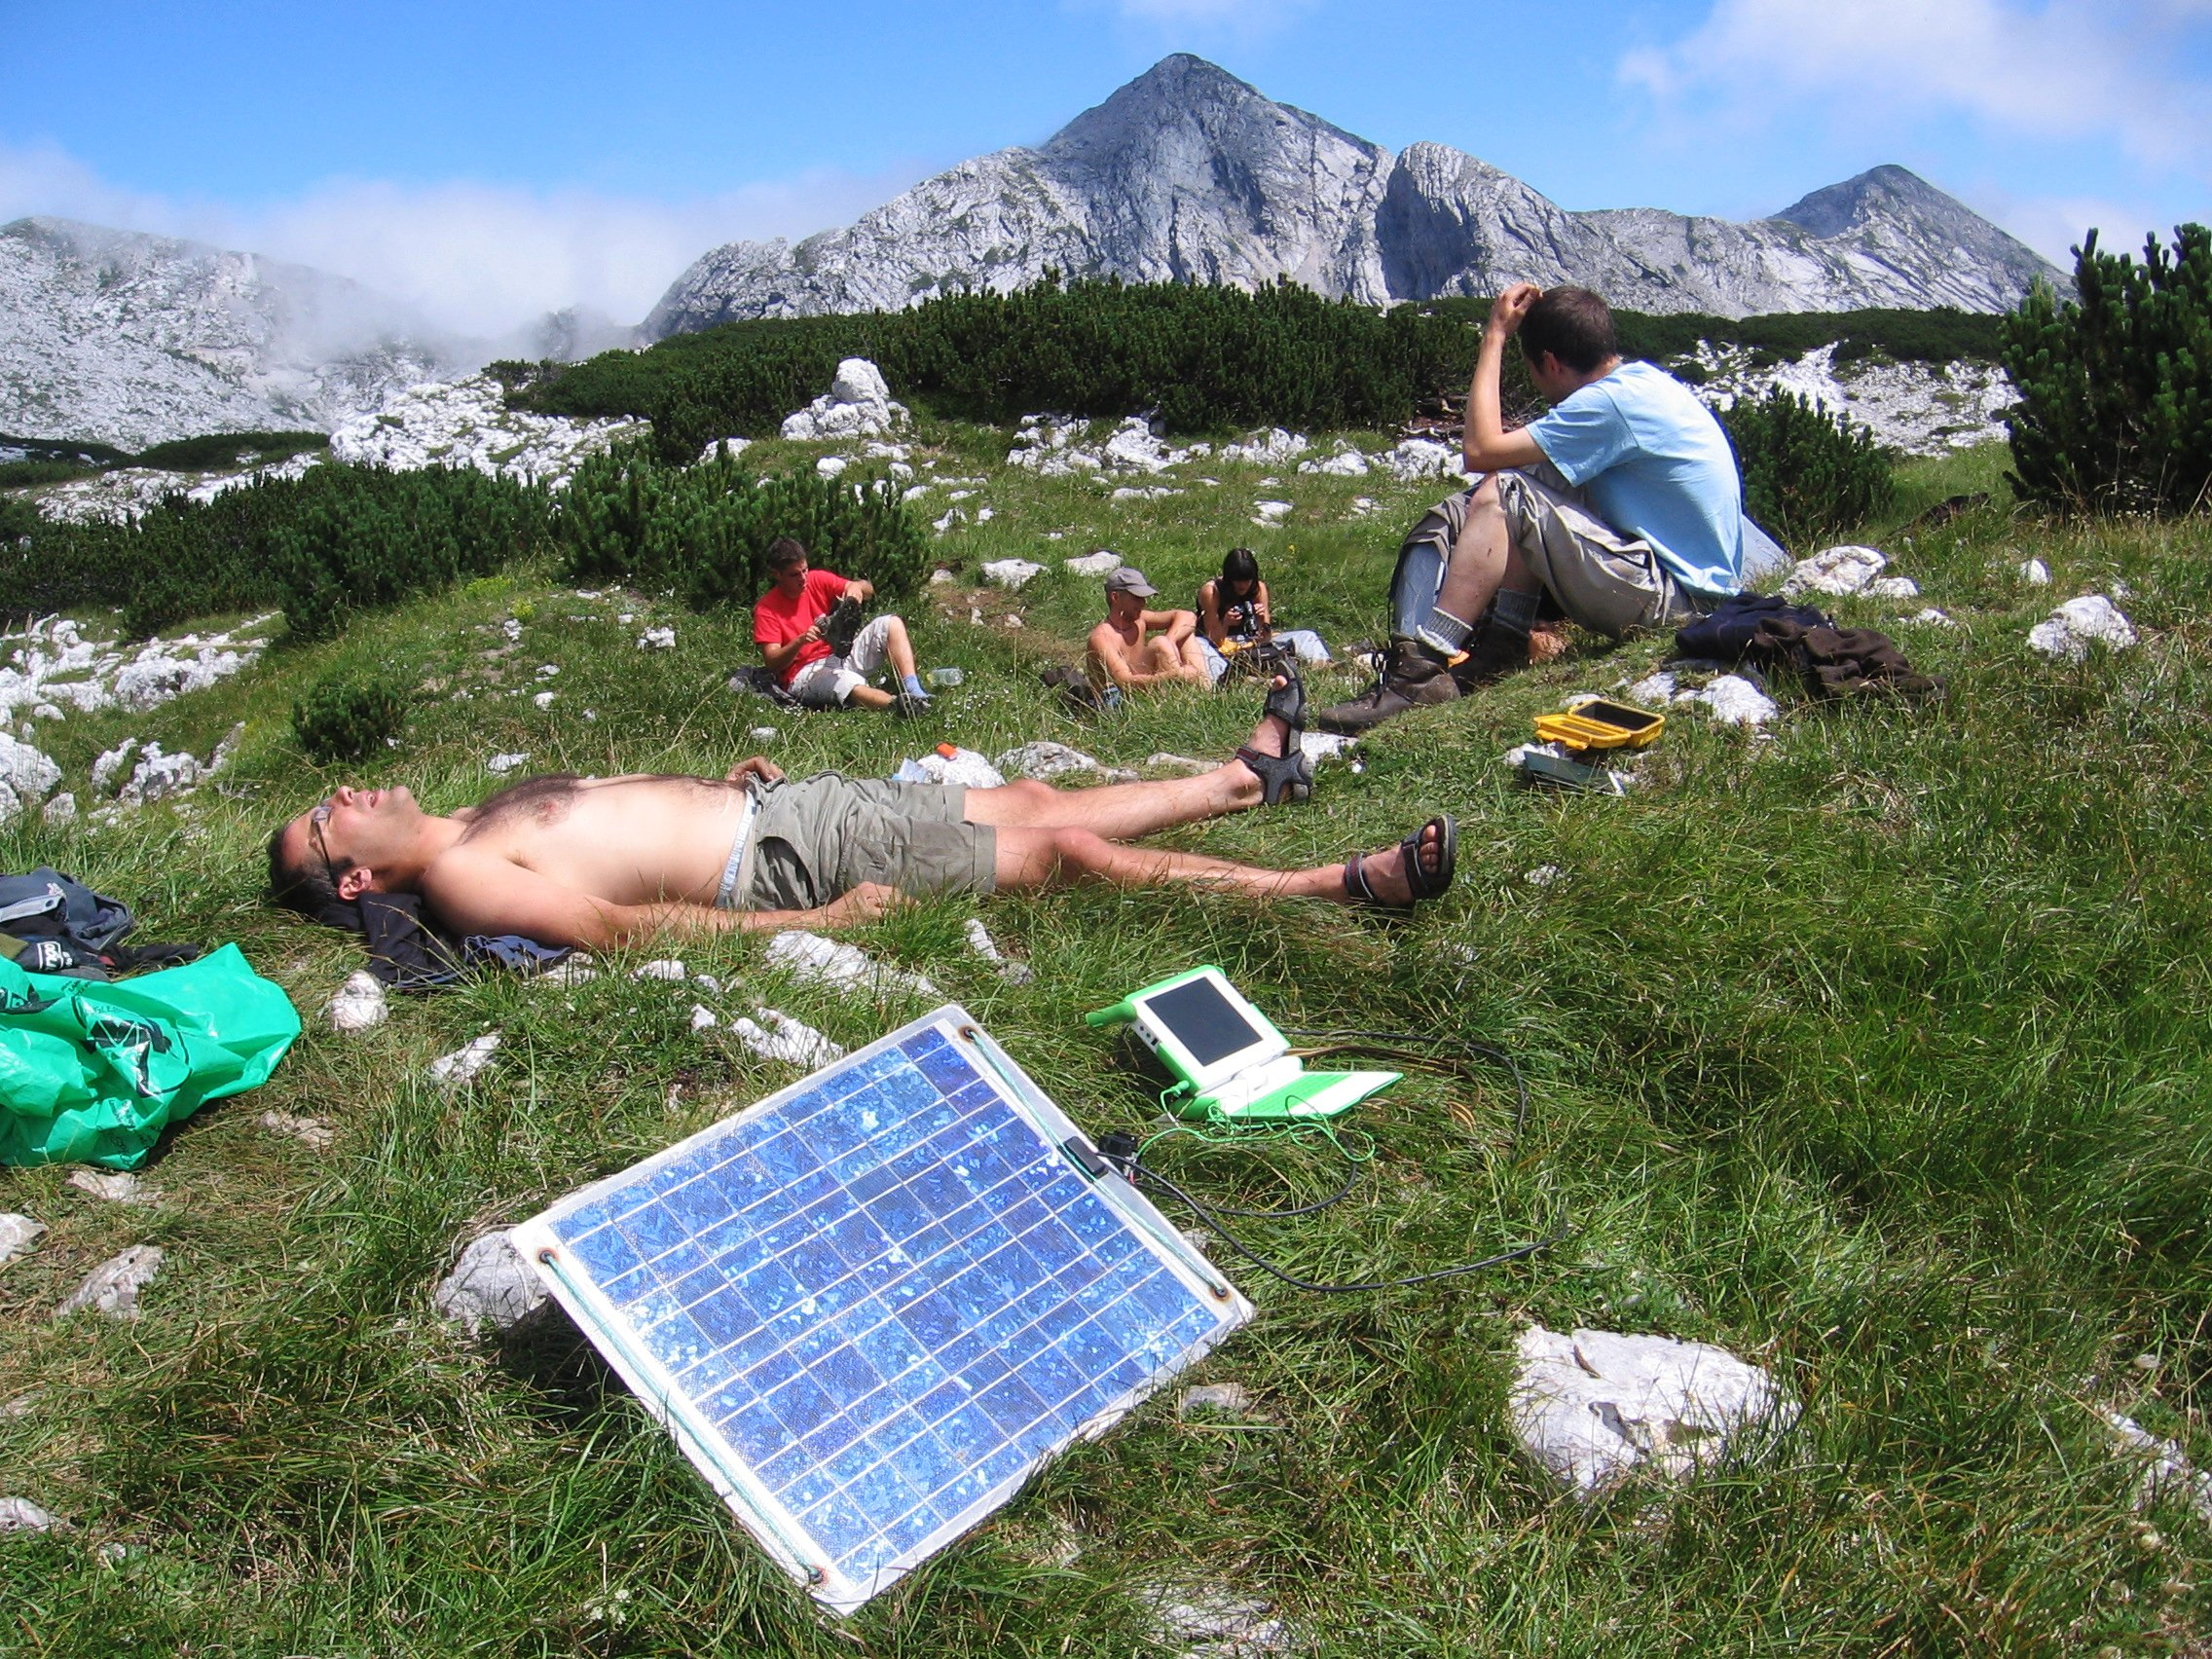
\includegraphics[width=\linewidth]{2008/diary/Jarvist Frost - canon a520 - faff on the plateau with a laptop--orig.jpg}}
\caption{The expedition laptop is one of the most important pieces of equipment. Here, cavers relax while the sunshine charges the laptop battery. \pic{Jarvist Frost}}
\end{marginfigure}


As such, attention shifted to higher leads to try and secure a
connection in 2008. From the \passage{Something Fishy} chamber a series of
pitches were explored which included the impressive \passage{Dangermouse}. The leads at the bottom are rather dubious, but it makes an
extremely pleasant 72m shaft series (Penfold, Dangermouse, Green
Back, Giblet Breakfast) which has a very valuable commodity on it indeed
- a seemingly faithful stream enters halfway down \passage{Dangermouse} and
collects in a secluded 2 m diameter plunge pool.

The \passage{Captain Kangaroo} series is extraordinarily dry after
\passage{Bonus Chamber} (it is actual dust, not water vapour, that ruins
flash photos in this part of the cave), and the water on
\passage{Dangermouse} is likely to be an important part of future
underground camping plans for 2009.

From \passage{Kill'em All}, a number of avens are noted. One of these was
gained by a rather gung-ho climb with uncertain belay to reach rift that
led away from the pitch. On a future trip, the rigging was improved to
an acceptable level and the rift was pushed to a squeeze. This soon gave
in to hammer attack, and led on to a initially upsetting pitch head.
There was clearly something big and echoing below, but the pitch head
was initially a fair squeeze for an anorexic cat! Disturbingly,
considering it was also our floor, the rock around the pitch head
shattered easily and with a few hours of work produced something
probably passable. The rotten nature of the rock was a concern when
placing the belays, and gained this section of cave the name
\passage{Cheesecake}. A short 10 meter pitch dropped onto an epic rock
bridge in a large chamber, with shafts disappearing down (perhaps
combining below) on either side with multiple second free falls. A
notable rift led off South (towards \passage{M2}) from the far side of the
chamber, but required a bolt traverse out to it. By survey, this rock
bridge is 21 meters directly above \passage{Dark Tranquillity}, so it
is likely that at least one of the pitches connects.


\begin{marginfigure}
\checkoddpage \ifoddpage \forcerectofloat \else \forceversofloat \fi
\centering
 \frame{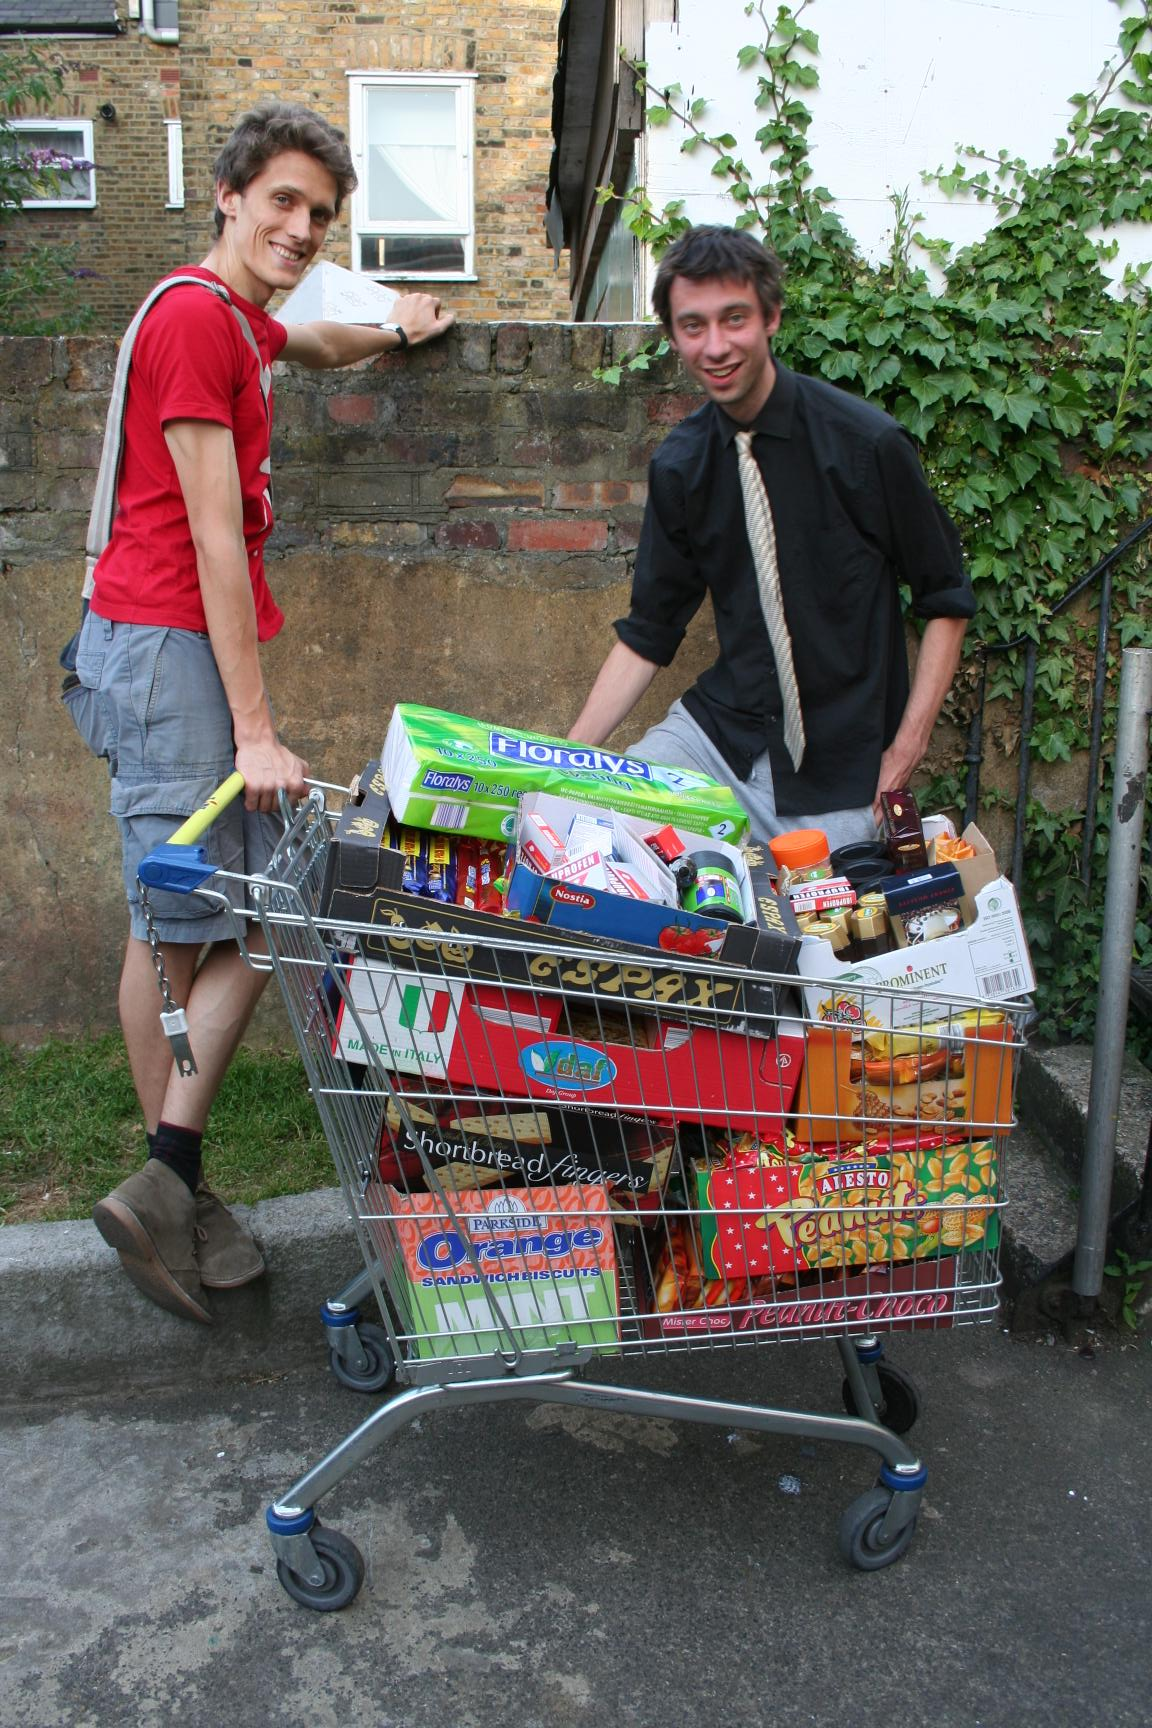
\includegraphics[width=\linewidth]{2008/diary/lidl.jpg}} 
 \caption{Several food purchases are made in the UK during run-up to expedition, sometimes months beforehand - but the final physical shop is never a one-man job. \pic{unknown}}
 \label{lidl food}
\end{marginfigure}



Due to a shortage of gear, a trip was made down the `\passage{Olympic
Rift}' arm of \passage{Captain Kangaroo} to recover equipment and scavenge
rope from the (left rigged since 2007) pitches. The exploration end was
a tight rift leading to a very large space, most likely a re-connection
to the \passage{Space Odyssey} / \passage{Concorde} pitch in the main \passage{Vrtnarija} shaft
series. An unsuccessful attempt was made on the squeeze - it required
expanding. The pitches were derigged and the rope removed to the bone
dry \passage{Traverse Chamber} for immediate use in 2009.

In this region a surface dig started and quickly broke into considerable
passage with a large draft. This was pushed very actively for a number
of trips, before an unfortunate connection being found into \passage{Jelly
Chamber} of \passage{Vrtnarija}. As the explorers at the time commented
``Well, at least its 800 m deep now!''. This \passage{Vilinska Jama} entrance
demonstrates the worth of spending time and effort on surface
excavations, as well as pointing to the plausibility of checking all the
small side passages in established systems.

Above the \passage{Vrtnarija}/\passage{Vilinska} valley is a limestone
pavement that extends from beyond the entrance to \passage{M2}. Here a
surface cave, \passage{E1}, was discovered in 2007 with a $\approx$ 20
m entrance pitch. During 2008 some stones were excavated to an extremely
tight (sub human) sized pitch head blowing strongly. This will require
chemical persuasion to pass, but due to the (now surface surveyed)
location, is a cave of some interest for 2009. Strangely for a surface
cave it has some well defined cave formation (large meander), which
appears to have been saved from infill by an overhanging entrance and
position next to the edge of the plateau.

On the mountain we were joined for a couple of weeks by the younger
generation of the Slovenian JSPDT. The majority of their efforts were
directed to a cave on the Western edge of the plateau, gained by \bignote{a
rather jaw-dropping abseil} of 100 m into the mile-deep \passage{Tolminka} valley!
This cave \passage{Monatip}, whose entranced was noted in 2006 and exploration
begun in summer 2007, is very different in nature to the other mountain
caves, being mostly horizontal with the entrance at 1730 m appearing to
be a dried stream way. Monatip was extended to a total surveyed length
of 710 m, before connecting into the \passage{Primadona} / \passage{U-Bend}
system at -151 m. The exit via the easy \passage{Primadona} shaft system
was welcome!

It is unclear whether \passage{Monatip} will be revisited in the future.
Some of the original enthusiasm for its exploration was it heading
South-East into `blank mountain', but unfortunately it quickly developed
back towards the South-West and \passage{Primadona}. However, it certainly
indicates that \passage{Primadona} itself is a very fertile area for
further exploration.

\tweet{10:39PM Aug 8, 2008}{Mona connected to Primadona,making the western plateau caves ~3.7km long.Carried snow,which has provoked worst storm of expo! Jarv }

Also on the Western Plateau is \passage{Planika Jama}, discovered
simultaneously with \passage{Monatip}. Far more vertical in nature and
partially choked with snow, this was pushed to an ice filled chamber
with `phreatic like' blow holes through the ice. Unfortunately this
original chamber was not reached due to the shifting ice levels - lots
of snow fell in the Winter before the expedition, but also a lot of rain
in the spring. In \passage{Planika} this appeared to have drilled a 1 m
diameter hole through the initial snow plug which gained an icy vadose
development which dropped via a short pitch to a tight blowing rift.
Armed with only hammer and chisels, three cavers spent a full day
smashing this rift to reach a tight squeeze into a further chamber.
Exploration was left at this extremity. On another occasion, a window
noticed near a rebelay ledge was pushed (again necessitating the
expansion of tight rift) to gain a large chamber which actually went
higher than the original entrance to the cave.

In \passage{Sistem Mig}, a return was made to the pitch explored in 2007 named
\passage{Plopzilla} (P105 m). The objectives were to photograph the large
pitch, investigate the extension boulder choke on one side of the pitch,
and to derig the rope to \passage{NCB} for use in future years looking at
other possible shafts coming off this neglected area of the system. The
boulder choke was climbed down through for tens of meters, halting when
reaching a committing climb down through the ever unstable boulders.
Once everyone present had confirmed that ``it goes, but I'm not going
there'' they derigged. Unfortunately the long exposure film photographs
taken with the aid of manually fired flashes on abseiling into the shaft
were badly fogged, probably due to the camera not being so light tight
after its many caving trips! A great pity, as the shaft had a beautiful
fluted triangular-prism cross section.


\begin{marginfigure}
\checkoddpage \ifoddpage \forcerectofloat \else \forceversofloat \fi
\centering
 \frame{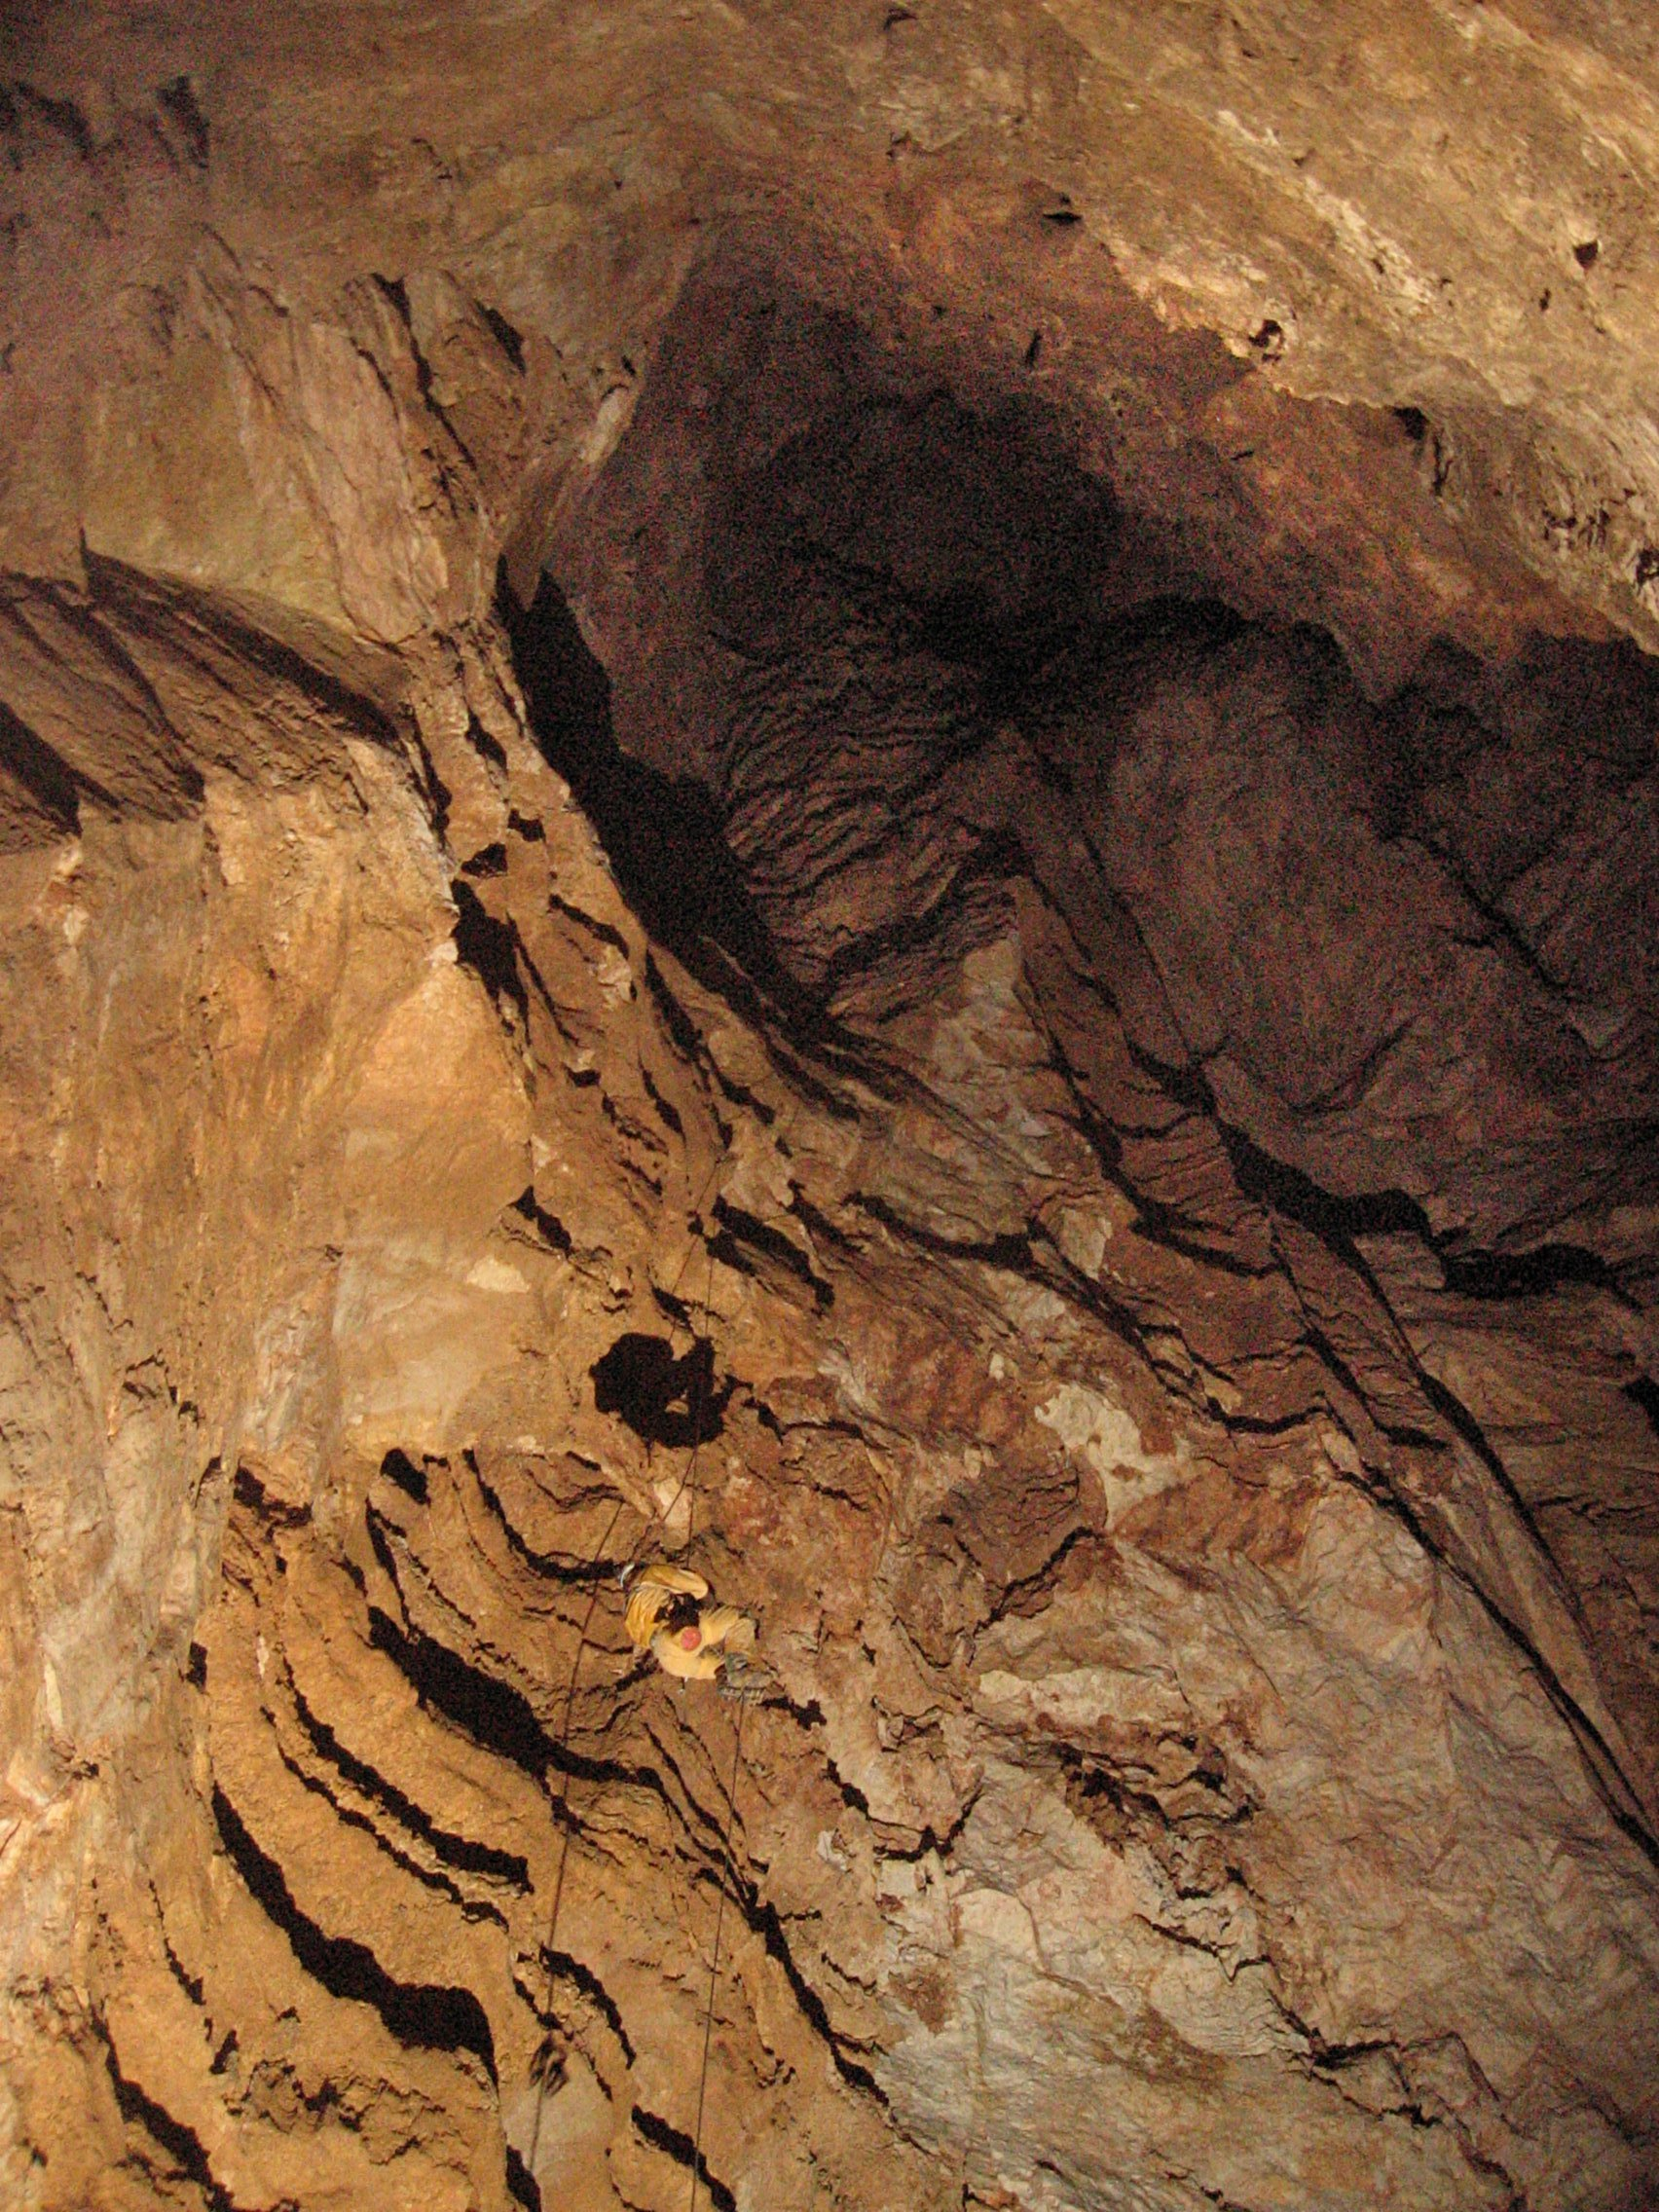
\includegraphics[width=\linewidth]{2008/diary/Jarvist Frost - canon a520 -plopzilla - looking up paul nearly at first rebelay--orig.jpg}} 
 \caption{Paul Hutton ascending \protect\passage{Plopzilla} pitch.  \pic{Jarvist Frost}}
 \label{paul plopzilla}
\end{marginfigure}


\passage{NCB} still holds interest for us, for though it was discovered in 1995
and provided the key for the discoveries of 1996, it has since been
visited rarely (due to its long distance in time from the surface).

A fair amount of surface prospecting has been concerned with investigating
the clear valley located on the mountain top above which contains the
small \passage{M15} and \passage{M17} caves. \passage{M17} was re-entered but found to be choked with
ice. Small caves were found nearby - initial digging has been started.